\documentclass[10pt, a4paper]{article}
\usepackage[top=1.8cm, bottom=1.8cm, left=1.8cm, right=1.8cm]{geometry}
\usepackage{amsmath, amssymb}
\usepackage{multicol}
\usepackage{enumitem}
\usepackage{titlesec}
\usepackage{xcolor}
\usepackage{booktabs}
\usepackage{array}
\usepackage{microtype}
\usepackage{parskip}
\usepackage{fancyhdr}
\usepackage{hyperref}
\usepackage{tikz}
\usetikzlibrary{arrows.meta, positioning}
\definecolor{ibmblue}{RGB}{15, 98, 254}
\definecolor{darkgray}{RGB}{60, 60, 60}
\titleformat{\section}{\normalfont\bfseries\color{ibmblue}\large}{}{0em}{}[\vspace{-0.3em}\rule{\linewidth}{0.8pt}]
\titlespacing*{\section}{0pt}{0.6em}{0.3em}
\titleformat{\subsection}{\normalfont\bfseries\color{darkgray}\normalsize}{}{0em}{}
\titlespacing*{\subsection}{0pt}{0.4em}{0.15em}
\setlist[itemize]{noitemsep, topsep=1pt, leftmargin=1.2em}
\setlist[enumerate]{noitemsep, topsep=1pt, leftmargin=1.4em}
\pagestyle{fancy}
\fancyhf{}
\renewcommand{\headrulewidth}{0pt}
\fancyhead[L]{\small\color{darkgray}\textit{Quantum Computing SOP --- Weekly Summary}}
\fancyhead[R]{\small\color{darkgray}\textit{Week 3}}
\fancyfoot[C]{\small\color{darkgray}\thepage}
\hypersetup{colorlinks=true, linkcolor=ibmblue, urlcolor=ibmblue}
\begin{document}
\begin{center}
  {\LARGE\bfseries\color{ibmblue} Week 3: Quantum Computing Workflow}\\[0.4em]
  {\large The Qiskit Pattern: Map $\to$ Optimize $\to$ Execute $\to$ Post-process}\\[0.3em]
  {\small\href{https://quantum.cloud.ibm.com/docs/en/guides/intro-to-patterns}{\texttt{quantum.cloud.ibm.com/docs} --- Development Workflow (Intro to Patterns)}}
\end{center}
\vspace{0.3em}
\hrule height 1.2pt
\vspace{0.4em}
\begin{center}
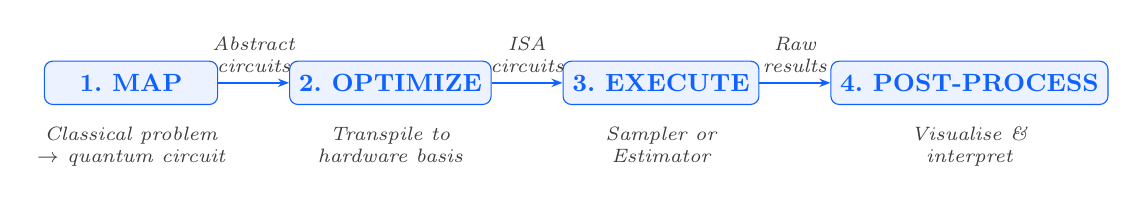
\begin{tikzpicture}[
  node distance=0.6cm and 0.9cm,
  box/.style={draw=ibmblue, rounded corners=3pt, fill=ibmblue!8,
              minimum width=2.2cm, minimum height=0.55cm,
              font=\small\bfseries, text=ibmblue, align=center},
  arr/.style={-{Stealth[length=4pt]}, ibmblue, thick},
  lbl/.style={font=\scriptsize\itshape, text=darkgray, align=center}]
  \node[box] (map)  {1.\ MAP};
  \node[box, right=of map]  (opt)  {2.\ OPTIMIZE};
  \node[box, right=of opt]  (exe)  {3.\ EXECUTE};
  \node[box, right=of exe]  (post) {4.\ POST-PROCESS};
  \draw[arr] (map)  -- node[above,lbl]{Abstract\\circuits} (opt);
  \draw[arr] (opt)  -- node[above,lbl]{ISA\\circuits}      (exe);
  \draw[arr] (exe)  -- node[above,lbl]{Raw\\results}       (post);
  \node[lbl, below=0.15cm of map]  {Classical problem\\$\to$ quantum circuit};
  \node[lbl, below=0.15cm of opt]  {Transpile to\\hardware basis};
  \node[lbl, below=0.15cm of exe]  {Sampler or\\Estimator};
  \node[lbl, below=0.15cm of post] {Visualise \&\\interpret};
\end{tikzpicture}
\end{center}
\vspace{0.3em}
\begin{multicols}{2}
\section{Step 1 --- Map}
Translate a \textbf{classical domain problem} into quantum circuits and/or operators.
\begin{itemize}
  \item Build \texttt{QuantumCircuit} objects encoding the problem
  \item Specify observables as \texttt{SparsePauliOp} (for Estimator)
  \item Decide output type: \emph{bitstrings} (Sampler) or \emph{expectation values} (Estimator)
\end{itemize}
\noindent\textbf{Bell state mapping:}
\[
  |00\rangle \xrightarrow{H \otimes I} \tfrac{|0\rangle+|1\rangle}{\sqrt{2}}|0\rangle
  \xrightarrow{\text{CNOT}} \frac{|00\rangle+|11\rangle}{\sqrt{2}} = |\Phi^+\rangle
\]
\noindent\textbf{Parameterised ansatz for VQE:}
\[
  \langle H\rangle = \langle\psi(\boldsymbol\theta)|ZZ + 0.5\,XI|\psi(\boldsymbol\theta)\rangle
\]

\section{Step 2 --- Optimize (Transpile)}
Convert the abstract circuit to an \textbf{ISA (Instruction Set Architecture) circuit}:
\begin{enumerate}
  \item \textbf{Gate decomposition} --- rewrite in hardware basis (\texttt{rz}, \texttt{sx}, \texttt{cx})
  \item \textbf{Routing} --- insert SWAPs to respect the coupling map
  \item \textbf{Optimization} --- cancel redundant gates, reduce depth
\end{enumerate}
\begin{center}
\renewcommand{\arraystretch}{1.15}
\begin{tabular}{ccc}
\toprule
\textbf{Level} & \textbf{Description} & \textbf{Use case}\\
\midrule
0 & No optimisation & Debug\\
1 & Light            & Quick runs\\
2 & Medium           & General\\
3 & Heavy            & Real hardware\\
\bottomrule
\end{tabular}
\end{center}
Observables must be remapped after transpilation:\\
\centerline{\texttt{H\_isa = H.apply\_layout(circuit\_isa.layout)}}

\section{Step 3 --- Execute}
Run ISA circuits using one of the two primitives:
\begin{center}
\renewcommand{\arraystretch}{1.15}
\begin{tabular}{p{1.7cm}p{2.1cm}p{1.5cm}}
\toprule
\textbf{Primitive} & \textbf{Output} & \textbf{Use case}\\
\midrule
\textbf{Sampler}   & Bitstring counts & Grover's, QFT\\
\textbf{Estimator} & $\langle O\rangle$ values & VQE, QAOA\\
\bottomrule
\end{tabular}
\end{center}
\noindent\textbf{Execution modes} (real hardware):
\begin{itemize}
  \item \textbf{Session} --- reserved QPU connection; ideal for iterative algorithms
  \item \textbf{Batch} --- parallel job submission; ideal for parameter sweeps
\end{itemize}

\section{Step 4 --- Post-process}
Interpret raw primitive outputs:
\begin{itemize}
  \item Plot bitstring histograms and probability distributions
  \item Apply readout-error mitigation techniques
  \item Marginalise distributions to smaller qubit subsets
  \item Postselect on physical constraints (parity, spin, particle number)
  \item Feed $\langle H\rangle$ to a classical optimiser (VQE loop)
\end{itemize}

\section{Experiments}
\subsection{A --- Bell State $|\Phi^+\rangle$ (Sampler)}
1024 shots via \texttt{BackendSamplerV2}. Only $|00\rangle$ and $|11\rangle$ appear:
\[P(|00\rangle)+P(|11\rangle)\approx 1.00\]
Confirms maximal two-qubit entanglement.

\subsection{B --- Pauli Observable (Estimator)}
Parameterised ansatz evaluated over four $\boldsymbol\theta$ configurations. Energy landscape $\langle ZZ+0.5\,XI\rangle$ visualised --- foundation of VQE.

\subsection{C --- GHZ State (Full Pattern)}
\[|GHZ\rangle=\tfrac{1}{\sqrt{2}}\bigl(|000\rangle+|111\rangle\bigr)\]
2048 shots; only $|000\rangle$ and $|111\rangle$ observed, confirming maximal 3-qubit entanglement.

\section{Qiskit Tools Used}
\begin{itemize}
  \item \texttt{QuantumCircuit}, \texttt{SparsePauliOp}, \texttt{ParameterVector}
  \item \texttt{generate\_preset\_pass\_manager} (levels 0--3)
  \item \texttt{BackendSamplerV2}, \texttt{BackendEstimatorV2}
  \item \texttt{AerSimulator} --- local simulation (no IBM account)
  \item \texttt{.apply\_layout()} --- observable qubit remapping
\end{itemize}
\end{multicols}
\vspace{0.2em}
\hrule height 0.6pt
\vspace{0.3em}
\section*{\color{ibmblue}Key Takeaways}
\begin{multicols}{2}
\begin{enumerate}[label=\textbf{\arabic*.}]
  \item \textbf{ISA Circuits are Mandatory.} Hardware only understands its native gate set. The transpiler decomposes abstract gates and routes operations through the coupling map.
  \item \textbf{Sampler vs Estimator.} Sampler returns bitstring counts; Estimator returns expectation values. Choose based on what the algorithm requires as output.
  \item \textbf{Observable Layout Must Match.} After transpilation, always call \texttt{.apply\_layout()} on your observable to keep qubit indices consistent with the physical mapping.
  \item \textbf{Higher Optimization = Fewer Gates.} Level 3 cuts gate count significantly over level 0, reducing noise on real hardware at the cost of longer classical compile time.
  \item \textbf{The Pattern is Modular.} Each step can be independently improved or swapped, enabling seamless integration of new tools and error-mitigation techniques.
\end{enumerate}
\end{multicols}
\end{document}